\documentclass[10pt]{scrartcl}

\usepackage[utf8]{inputenc}
\usepackage{tabularx}
\usepackage{longtable}
\usepackage[ngerman]{babel}
\usepackage[automark]{scrpage2}
\usepackage{amsmath,amssymb,amstext}
%\usepackage{mathtools}
\usepackage[]{color}
\usepackage[]{enumerate}
\usepackage{graphicx}
\usepackage{lastpage}
\usepackage[perpage,para,symbol*]{footmisc}
\usepackage{listings} 

\usepackage[numbers,square]{natbib}
\usepackage{color}
\usepackage{colortbl}
\usepackage[absolute]{textpos}
\usepackage{float}
\usepackage{verbatim}
\usepackage[colorinlistoftodos,textsize=small,textwidth=2cm,shadow,bordercolor=black,backgroundcolor={red!100!green!33},linecolor=black]{todonotes}

\usepackage[pdfborder={0 0 0},colorlinks=false]{hyperref}
\usepackage[all]{hypcap}


\lstset{numbers=left, numberstyle=\tiny, numbersep=5pt, breaklines=true, showstringspaces=false} 
\restylefloat{figure}

%changehere
\def\titletext{Lab 2: SIP, Multicast}
\def\titletextshort{Praktikum 2}
\author{André Harms, Oliver Steenbuck}

\title{\titletext}

%changehere Datum der Übung
\date{04.01.2012}

\pagestyle{scrheadings}
%changehere
\ihead{TT1, Schmidt}
\ifoot{Generiert am:\\ \today}

\cfoot{Oliver Steenbuck, André Harms}


\ohead[]{\titletextshort}
\ofoot[]{{\thepage} / \pageref{LastPage}}

\setlength{\parindent}{0.0in}
\setlength{\parskip}{0.1in}

\begin{document}
\maketitle

\setcounter{tocdepth}{3}
\tableofcontents

%	\listoftables                                 												% 
%	\listoffigures   

\section{Durchführung des Versuchs}

\subsection{Versuchsaufbau}\label{subsec:versuchsaufbau}
Der Versuch wurde mit der Gruppe Noetzel/Steude zusammen durchgeführt.
Es wurde pro Gruppe auf einem Rechner der Client gestartet, ein Server wurde nur auf dem Rechner der Gruppe Harms/Steenbuck gestartet. Die IP Adressen der am Versuch beteiligten entsprechenden Rechner waren:
\begin{description}
	\item[Noetzel/Steude] \verb!141.22.27.34!
	\item[Harms/Steenbuck] \verb!141.22.27.35!
	\item[SIP Gateway] \verb!141.22.27.3!
\end{description}

\subsection{Versuchsablauf}
Der Versuch sollte sowohl die SIP Funktionalität der jeweiligen Implementierungen als auch das IGMP Netzwerk im Labor testen. Um diese Ziele zu erreichen wurde folgendes Vorgehen (aus Sicht Server: Steenbuck/Harms) gewählt:

\begin{enumerate}
	\item \verb!Register! beim Proxy
	\item \verb!Invite! durch Client Noetzel/Steude
	\item \verb!Invite! durch Client Steenbuck/Harms
	\item \verb!Bye! durch Client Noetzel/Steude
	\item \verb!Bye! durch Steenbuck/Harms
	\item Server Stop
\end{enumerate}

Während des gesamten Versuchablaufes wurde der Netzwerkverkehr aufgezeichnet um diesen später auszuwerten, siehe \ref{sec:beobachtung}.
	
\section{Beobachtung} \label{sec:beobachtung}

\subsection{SIP}

\subsection{IGMP}

	\subsection{Join}
	
	
	\subsubsection{Message Pakete}
	
	\subsubsection{Leave}
	
	
	\subsection{Besonderheiten}
	
	Die Ergebnisse auf der IGMP Seite der Anwendung entsprechen den Erwartungen (\verb!join! nach \verb!invite! und \verb!leave! nach \verb!bye! auf Clientseite sowie analog auf der Serverseite das starten/stopen des sendens)
	
	Die einzige Ausnahme ist das nach dem clientseitigen \verb!leave! festgestellt wurde das wie weiterhin \verb!UDP Multicast! Nachrichten empfangen wurde, siehe Abbildung \ref{img:cap1}. 
	Die Erklärung hierfür dürfte sein, dass die Infrastrutkur in den Laborräumen kein IGMP Snooping unterstützt und daher die Multicastnachrichten über Ethernet Broadcasts implementiert. Diese kommen dann auch bei dem nicht in der Gruppe registriertem Rechner an.
	
	
	\begin{figure}[htb]
        \centering
         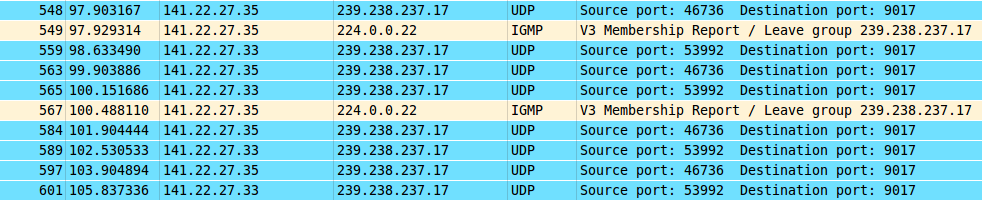
\includegraphics[width=\textwidth]{img/udp_after_leaving}
         \caption{Empfang von UDP Nachrichten nach Austritt aus Multicastgruppe}
        \label{img:cap1}
	\end{figure}	



\section{Bedienung der Anwendung}
\begin{enumerate}
	\item entpacken \verb!harmsSteenbuckSIP.tgz!
	\item wechseln in das Verzeichnis \verb!dist!
	\item \verb!java -jar "SIPGUI.jar"!
	\item Die unter \ref{sec:bedienung:anwendung} beschrieben Anwendung startet
\end{enumerate}


\label{sec:bedienung:anwendung}		
	\begin{figure}[H]
        \centering
                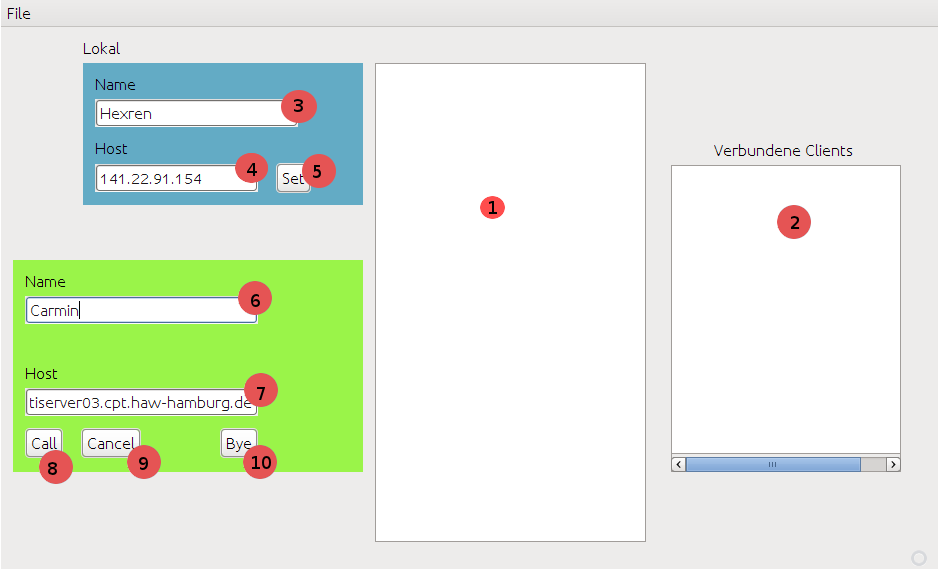
\includegraphics[width=\textwidth]{img/screenshotApplication}
        \caption{Screenshot der GUI}
        \label{img:gui}
	\end{figure}

\begin{enumerate}
	\item Bereich in dem die empfangenen IGMP Nachrichten angezeigt werden
	\item Zum Server verbundene Clients
	\item Name mit dem sich beim Proxy registriert wird
	\item IP Adresse des Rechners
	\item Knopf zum Registrieren
	\item Name des zu invitenden Teilnehmers
	\item IP Adresse des zu invitenden Teilnehmers
	\item Knopf zum Anrufen (inviten) des in X angegebenen Teilnehmers
	\item Knopf zum Abbrechen eines Invites
	\item Knopf zum Beenden der Verbindung
\end{enumerate}

\section{Sourcen}
Das Project besteht im wesentlichen asu 2 teilen. Zum ersten eine Bibliothekt die SIP und IGMP funktionalitäten bietet und in Eclipse mit Maven entwickelt wurde zum anderene ine Oberfläche die in Netbeans entwickelt wurde und die Bibliothek nutzt. In den Sourcen sollte sich seit der Abgabe nichts mehr geändert haben, im zweifelsfall ist der commit \verb!fd4d802c26! der letzte vor der Abgabe gewesen.

Die Sourcen für beide Projekte sind auf githup unter folgenden Pfaden verfügbar.
\begin{description}
	\item[Bibliothek] Eclipse \\ \verb!https://github.com/MyersGer/WS_2011/tree/master/TT1/Prak2/lab3!
	\item[Oberfläche] Netbeans \\ \verb!https://github.com/MyersGer/WS_2011/tree/master/TT1/Prak2/guiHarmsSteenbuck!
\end{description}

\section{Anlagen}
\begin{itemize}
	\item ausführbare Jar
\end{itemize}

\end{document}

